\section{Latar Belakang}

Pengembangan agen otonom untuk memecahkan permasalahan algoritmik maupun fisis merupakan studi yang populer seiring berkembangnya sumber daya komputasi yang semakin kuat. Salah satu kerangka pengembangan agen otonom yang marak digunakan adalah \acf{RL}. \ac{RL} merupakan kerangka pengembangan agen otonom yang berbasis strategi/kebijakan yang dapat dilatih tanpa supervisi. Pengembangan agen otonom menggunakan \ac{RL} dapat dideskripsikan oleh diagram gambar \ref{fig:RL-diagram}

\begin{figure}[h]
	\centering
	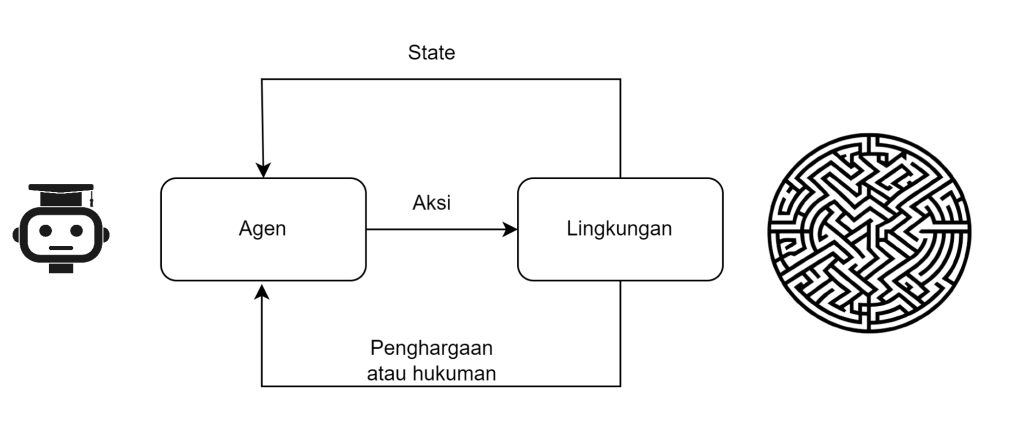
\includegraphics[width=0.8\textwidth]{chapter-1/diagram-RL.png}
	\caption{Diagram \acl{RL}}
	\label{fig:RL-diagram}
\end{figure}

\ac{RL} berperan sebagai pembaru strategi yang belajar dari pengamatan yang didapat sebagai hasil dari aksi yang dilakukan oleh agen. Sehingga, agen dapat melakukan aksi yang dianggap lebih baik. Aksi yang lebih baik dinilai dari hasil yang didapatkan, apabila aksi dinilai baik maka \ac{RL} akan mendapat penghargaan sehingga membuat aksi yang diambil akan memiliki probabilitas terjadi lebih besar ketika diberi hasil observasi yang sama. Sebaliknya, apabila aksi dinilai buruk maka \ac{RL} akan mendapatkan hukuman sehingga membuat aksi yang diambil akan memiliki probabilitas terjadi lebih kecil ketika diberi hasil observasi yang sama.

\ac{RL}, sebagai pembaru strategi, dapat digunakan sebagai solusi pada permasalahan domain khusus yang memiliki dinamika yang terlalu sulit untuk dimodelkan tetapi masukan dan keluaran dari sistem terdefinisi secara terbatas. Beberapa studi sebelumnya, telah menggunakan RL untuk menyelesaikan berbagai permasalahan seperti robotika kawanan \parencite{hubert2022perancangan}, agen perencana jalur \parencite{dawne2023algoritma}, dan agen pengemudi kendara otonom \parencite{mardhatillah2023strategi}. Permasalahan-permasalahan tersebut terkait erat dengan domain perangkat keras karena hasil implementasi RL akan kemudian digunakan pada agen otonom yang berbasis komputer.

Salah satu model utama yang digunakan untuk merilis model RL kepada sebuah perangkat keras dengan sumber daya terbatas adalah \ac{EC}. \ac{EC} merupakan sebuah alternatif model komputasi yang menggunakan awan, kluster komputer yang digunakan sebagai daya komputasi utama. Permasalahan dengan konsep komputasi awan adalah munculnya waktu tunda dari latensi komunikasi antara perangkat keras pengguna dan komputer awan. Ide utama dari \ac{EC} adalah memindahkan daya komputasi utama dari awan menjadi lebih dekat dengan pengguna sehingga latensi komunikasi akan tereduksi \parencite{edgecomputing}. Model rilis ini sesuai dengan RL karena dengan tereduksinya latensi maka sistem dapat merespon sebuah gangguan secara \textit{real-time}. Pada sistem \ac{EC}, yang tergambar pada gambar \ref{fig:edge-computing}, komputasi algoritma RL dapat dilakukan pada \textit{edge node} yang mampu melakukan komputasi lebih dengan \ac{IoT} \textit{node}.

\begin{figure}[h]
	\centering
	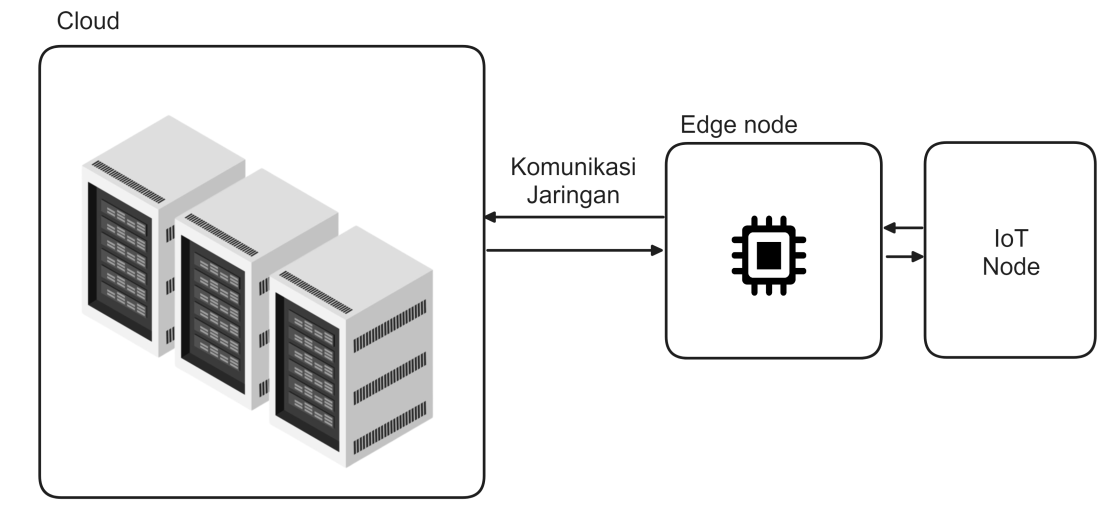
\includegraphics[width=0.8\textwidth]{chapter-1/edge-computing.png}
	\caption{Ilustrasi \acl{EC}}
	\label{fig:edge-computing}
\end{figure}

Namun, penggunaan model \ac{EC} memerlukan komputer di \textit{edge node} untuk dapat melakukan komputasi secara efektif tetapi hemat energi agar dapat digunakan dalam jangka waktu yang panjang dengan harga yang rendah. Hal ini merupakan tantangan untuk penggunaan model \ac{RL} karena umumnya model \ac{RL}, seperti \textit{soft critic}, itu menggunakan daya komputasi yang cukup besar sehingga memerlukan energi yang tinggi \parencite{wang2022efficient}.

Agar komputasi dapat dilakukan secara efektif tetapi menggunakan dapat lebih rendah, banyak teknik optimasi yang dapat digunakan. Salah satu teknik optimasi yang mampu mereduksi daya komputasi adalah dengan membuat akselerator perangkat keras khusus yang mampu melakukan komputasi RL secara lebih efisien. Efisiensi tersebut akan mengakibatkan komputer pada \textit{edge node} di gambar \ref{fig:edge-computing} dapat melakukan komputasi secara lebih optimal karena terdapat subsistem perangkat keras yang terdedikasi untuk melakukan perhitungan algoritma RL. Hal inilah yang melatari keinginan penulis untuk mengembangkan desain akselerator perangkat keras yang mampu melakukan komputasi RL secara lebih efektif dan efisien. Akselerator perangkat keras akan dirancang dengan berbasis pada arsitektur RISC-V, sebuah \textit{instruction set architecture} yang secara terbuka dikembangkan oleh RISC-V Foundation, dengan lisensi yang terbuka untuk dikembangkan sehingga memungkinkan untuk digunakan untuk riset tugas akhir.
